%\documentclass[a4paper,twocolumn]{article} % Document type
%       Compiler: pdflatex
% TODO: Task 2
% TODO: Task 3. Improved description of asymptotic stability. OBS! Still needs
% theoretical basis on why it is asymptotically stable.
% TODO: Task 4
% TODO: Task 5. FIXED
% TODO: Task 9
% TODO: Task 10
% TODO: Task 11
% TODO: Task 15
% TODO: Task 18
% TODO: Task 21
% TODO: Task 22

\documentclass[a4paper,12pt,oneside,onecolumn]{article} % Document type

\usepackage[left=1.0in, right=1.0in, top=1.0in, bottom=1.0in]{geometry}

\ifx\pdfoutput\undefined
    %Use old Latex if PDFLatex does not work
   \usepackage[dvips]{graphicx}% To get graphics working
   \DeclareGraphicsExtensions{.eps} % Encapsulated PostScript
 \else
    %Use PDFLatex
   \usepackage[pdftex]{graphicx}% To get graphics working
   \DeclareGraphicsExtensions{.pdf,.jpg,.png,.mps} % Portable Document Format, Joint Photographic Experts Group, Portable Network Graphics, MetaPost
   \pdfcompresslevel=9
\fi

\usepackage{amsmath,amssymb}   % Contains mathematical symbols
\usepackage[ansinew]{inputenc} % Input encoding, identical to Windows 1252
\usepackage[english]{babel}    % Language
\usepackage[square,numbers]{natbib}     %Nice numbered citations
\usepackage{siunitx}
\usepackage{graphicx}
\usepackage{float}
\bibliographystyle{plainnat}            %Sorted bibliography



\begin{document}               % Begins the document

\title{Homework 3 in EL2450 Hybrid and Embedded Control Systems}
\author{
  Martin Favre \\ 19920130-0010 \\ mfavre@kth.se 
  \and 
  Adam Lang \\ 19861110-3956 \\ adamlang@kth.se
  \and
  Andreas Fr\"oderberg \\ 19880730-7577 \\ andfro@kth.se
  \and
  }
%\date{2010-10-10}             % If you want to set the date yourself.

\maketitle                     % Generates the title


\section*{Task 1}


Given the equations 
	\begin{equation}
		u_\omega = \frac{u_r + u_l}{2}
	\end{equation}
	\begin{equation}
		u_\Psi = u_r-u_l,
	\end{equation}
and $u_\omega$ and $u_\Psi$, then $u_r$ and $u_l$ can be calculated as
	\begin{equation}
		u_r = u_\omega + \frac{u_\Psi}{2}
	\end{equation}
	\begin{equation}
		u_l =  u_\omega-\frac{u_\Psi}{2}
	\end{equation}
	
\section*{Task 2}

Using the generated data from Forward.csv and Rotate.csv, it is possible
to determine R and L. The data that is recieved, is time $[\mu$$s]$,
position x $[m]$, position y $[m]$ and rotation $\theta$$[^{\circ}]$.
%#JobbigasteTecknet2016

$\dot{x}$, $\dot{y}$ and $\dot{\theta}$ is calculated discretely. With
$R_1$ and $R_2$ and the input $\dot{x}$ and $\dot{y}$
as,
	\begin{equation}
		R_1 = \frac{\dot{x}}{cos(\theta)u_\omega}
	\end{equation}
	\begin{equation}
		R_2 = \frac{\dot{y}}{sin(\theta)u_\omega}
	\end{equation}
We can calculate $R$ as the mean value,
	\begin{equation}
		R = \frac{R_1 + R_2}{2}. % Övertydligt
	\end{equation}
L is determined simularily by calculating the mean values of from all
$\dot{\theta}$ with,
	\begin{equation}
		L =  \frac{R}{\dot{\theta}}u_\Phi
	\end{equation}
        Calculating these mean values will result in
	\begin{align*}
          &R = 5.2\\
          &L = 25.5\ \si{\milli\meter/\ang{1}}
	\end{align*}

\section*{Task 3}
Asymptotic stability means that for starting points close to an
equilibrium point, the system will asymptotically approach the equilibrium point
and stay there as the number of time units passed approach infinity. In a
practical sense, this means that the eigenvalues of the system are all confined
within the unit circle. Since this is the case for our system, we can say that
is it asymptotically stable.  Zeno behaviour is defined as an infinite amount of
state transitions in a finite amount of time. This is not valid in this case
since 
\begin{equation}
  \lim_{l \to \infty}\sum\limits_{l=1}^\infty t_i(s_i) \neq k
\end{equation}
where $s$ is a state transition, $t(s)$ is the function of the time 
for each state transitions and k is a constant.
This can also be seen in Figure \ref{fig:task3_plot}.
\begin{figure}[H]
    \centering
    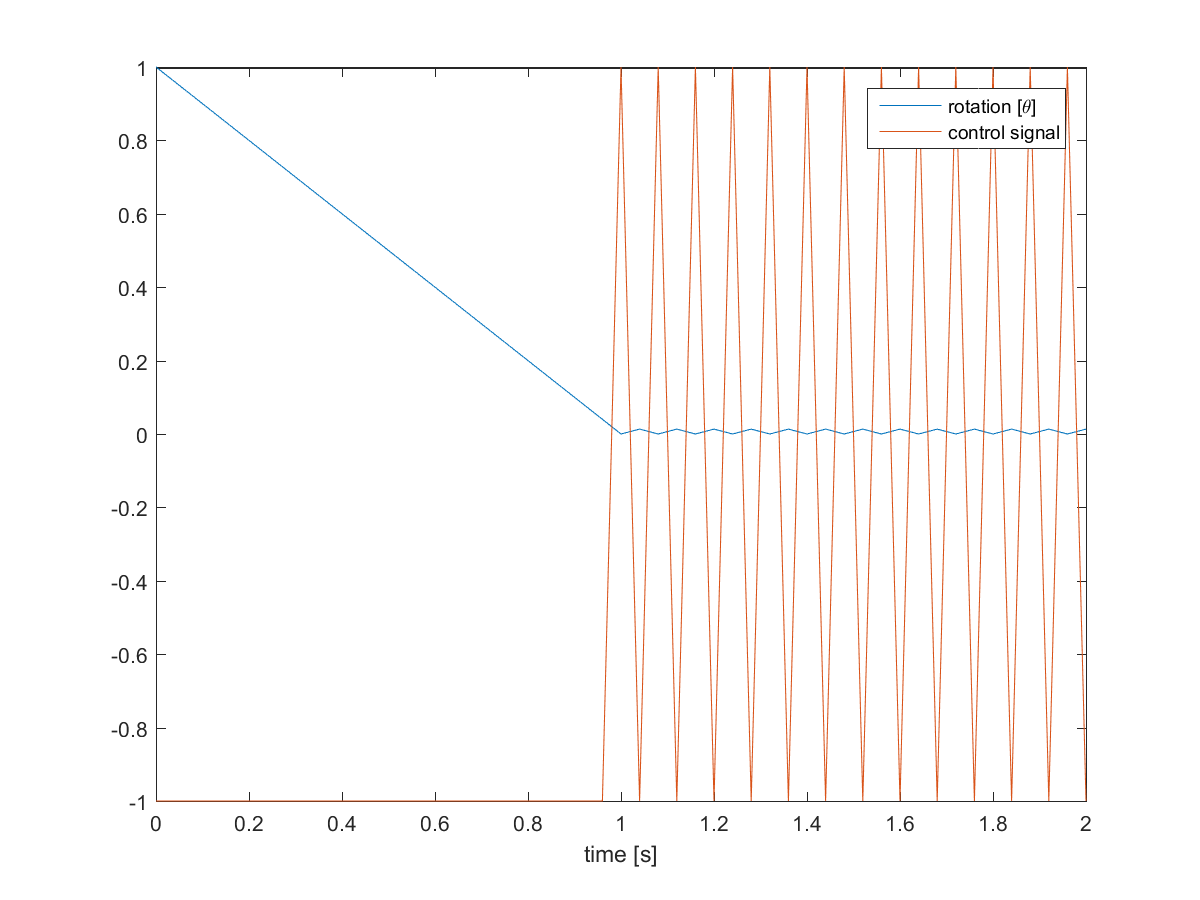
\includegraphics[scale=0.5]{../matlab/images/task3_plot.png}
    \caption{Response of rot1 simulink model.}
    \label{fig:task3_plot}
\end{figure}

\section*{Task 4}
Using the same definition as Task 3, we can say that the system
is asymptotically stable and in fact does exhibit Zeno
behaviour. In figure \ref{fig:task3_plot} the systems state
transitions approach infinite transitions in a finite amount of time. 
\begin{figure}[H]
    \centering
    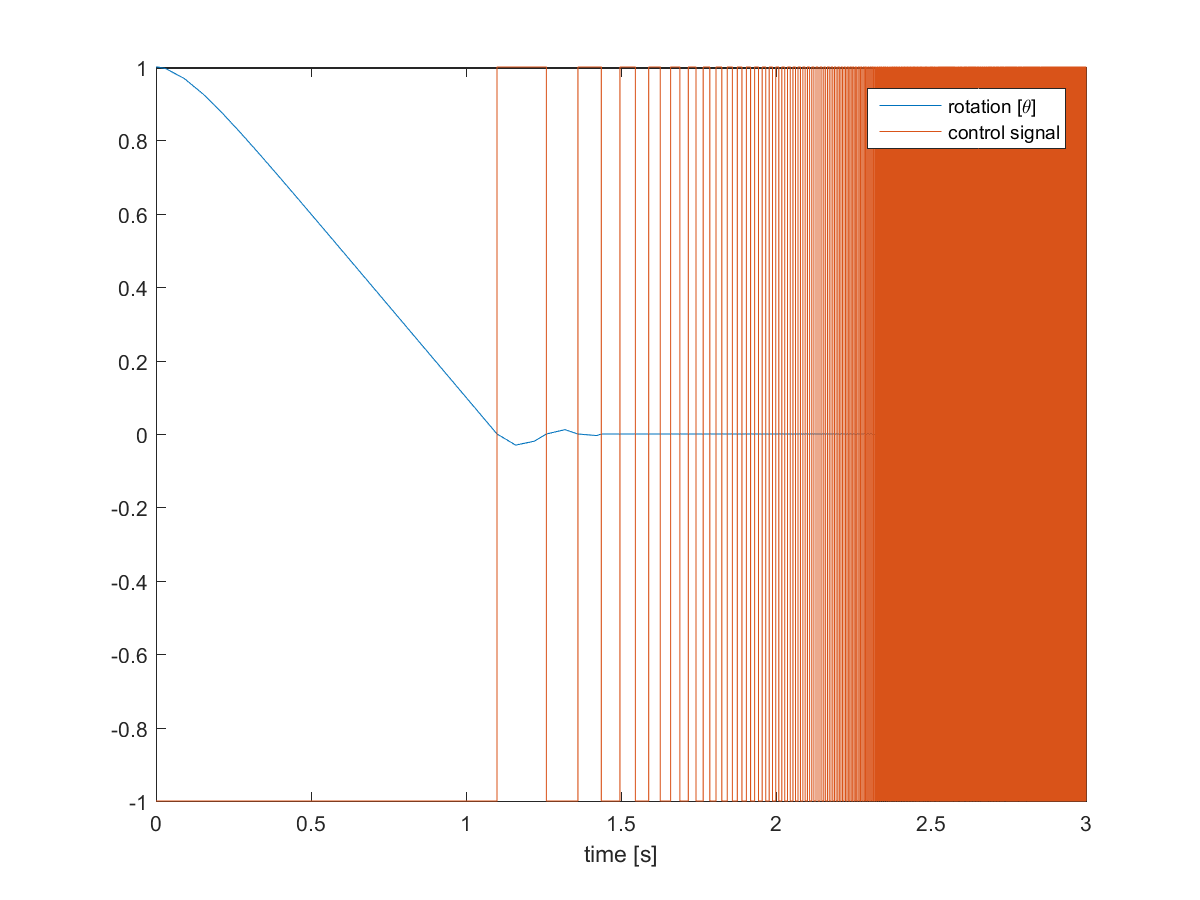
\includegraphics[scale = 0.5]{../matlab/images/task4_plot.png}
    \caption{Response of rot2 simulink model.}
    \label{fig:task4_plot}
\end{figure}
Even though this behaviour is asymptotically stable, it is not practical since a
physical system is limited in time and cannot switch infinitely many times.
\section*{Task 5}
The system system reaches an oscillating state where is stable, though no
asymptotically. The system does not have infinately many switches within a
finite time frame as in Task 4 and does as such  not exhibit Zeno behaviour. In
Figure~\ref{fig:task5_plot} the systems transitions per time unit reaches a
constant value. This is because of the added ZOH block in the model which limits
the response time of the system to once per sampling time of the ZOH, in this
case 0.01 s. 
\begin{figure}[H]
    \centering
    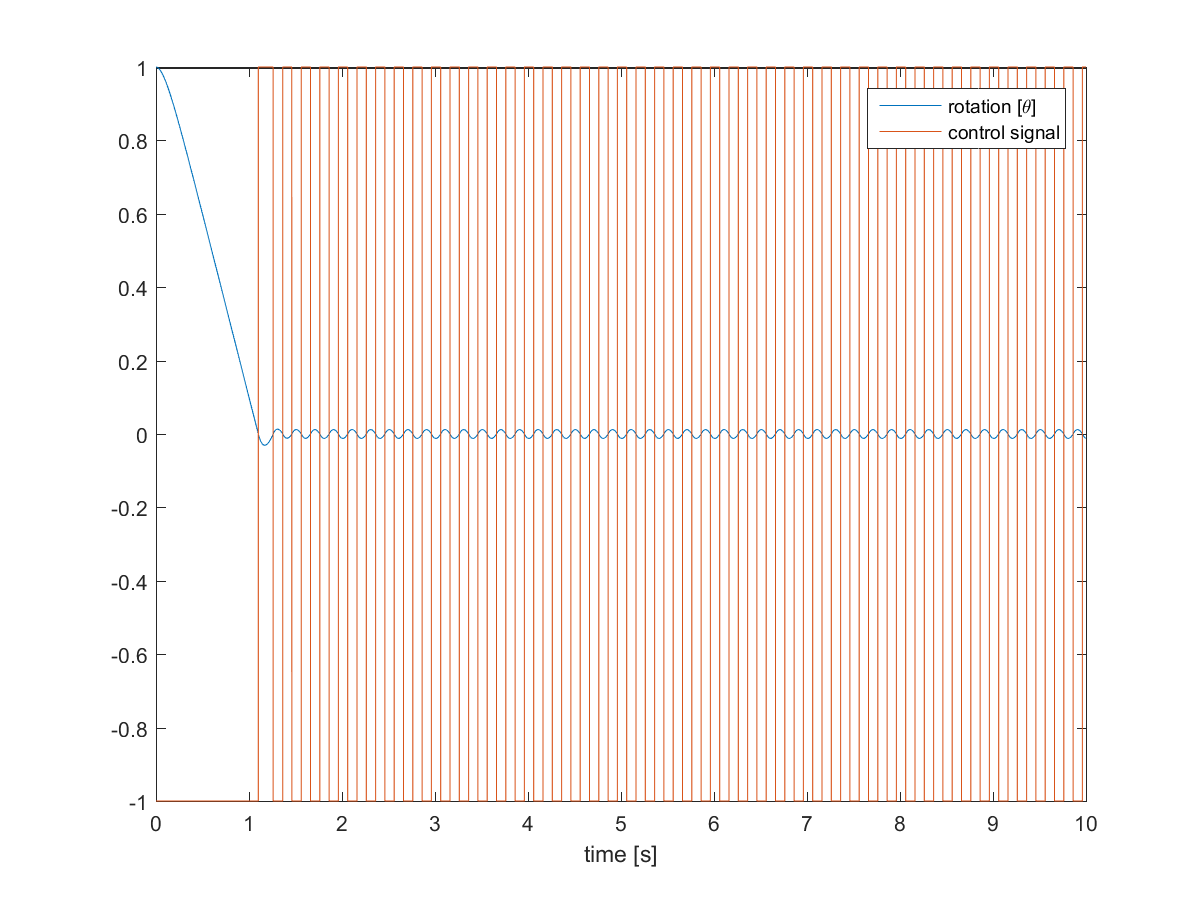
\includegraphics[scale = 0.5, width=1\linewidth]{../matlab/images/task5_plot.png}
    \caption{Response of rot3 simulink model.}
    \label{fig:task5_plot}
\end{figure}

\section*{Task 6}

Euler forward is a forward difference, in the $z$-transform written as
\begin{equation}
s = \frac{z-1}{\tau_s},
\end{equation}
where $s$ denotes the Laplace transform and the $z$-transform represents a time shift forward in the discrete domain. Applied to the dynamics of the $x$ variable, one yields
\begin{equation}
\frac{z-1}{\tau_s}x=Ru_\omega cos(\theta)
\end{equation}
which with similar calculations for all state variables yields the complete discrete system dynamics
\begin{equation}
\label{eq:xsystem}
x[k+h] = x[k] + \tau_s R u_\omega cos(\theta [k])	\\
\end{equation}
\begin{equation}
\label{eq:ysystem}
y[k+h] = y[k] + \tau_s R u_\omega sin(\theta [k]) \\
\end{equation}
\begin{equation}
\label{thetadynamics}
\theta[k+h] = \theta [k] + \frac{\tau_s R}{L} u_\psi.
\end{equation}


\section*{Task 7}
 	Given
	\begin{equation}
		\dot{\theta} = \frac{Ru_\Psi}{L}
		 \label{eq:thetadot}
	\end{equation}
	and
	\begin{equation}
		u_\Psi{[k]} = K_{\Psi}({\theta}^R  - {\theta}[k]).
	\end{equation}
	With Euler forward equation (~\ref{eq:thetadot}) gives
	\begin{equation}
		\theta[k+h] = \dot{\theta}[k]\tau_s + \theta[k]
	\end{equation}
	\begin{equation}
		\theta[k+h] = \frac{RK\tau_s({\theta}^R  - {\theta}[k])}{L} + \theta[k]
	\end{equation}
	\begin{equation}
R2 = R2 + R(1,i)^2;		\theta[k+h] =\theta[k](1-\frac{RK\tau_s}{L}) + \frac{RK_p\theta^R\tau_s}{L}
	\end{equation}
The eigenvalues are
	\begin{equation}
		\lambda = \left|{(1-\frac{RK\tau_s}{L})}\right| < 1
	\end{equation}
	which gives that 
	\begin{equation}
		0 < K < \frac{2L}{R\tau_s}
	\end{equation}

\section*{Task 8}
    The simulated task chosen was to rotate from $\theta = 0$ to $\theta = 90$.
    The angular response can be seen in Figure~\ref{fig:task8_angleplot}. The
    position's response can be seen inFigure~\ref{fig:task8_posplot} and shows
    that the position does not change.  \begin{figure}[H]
        \centering
        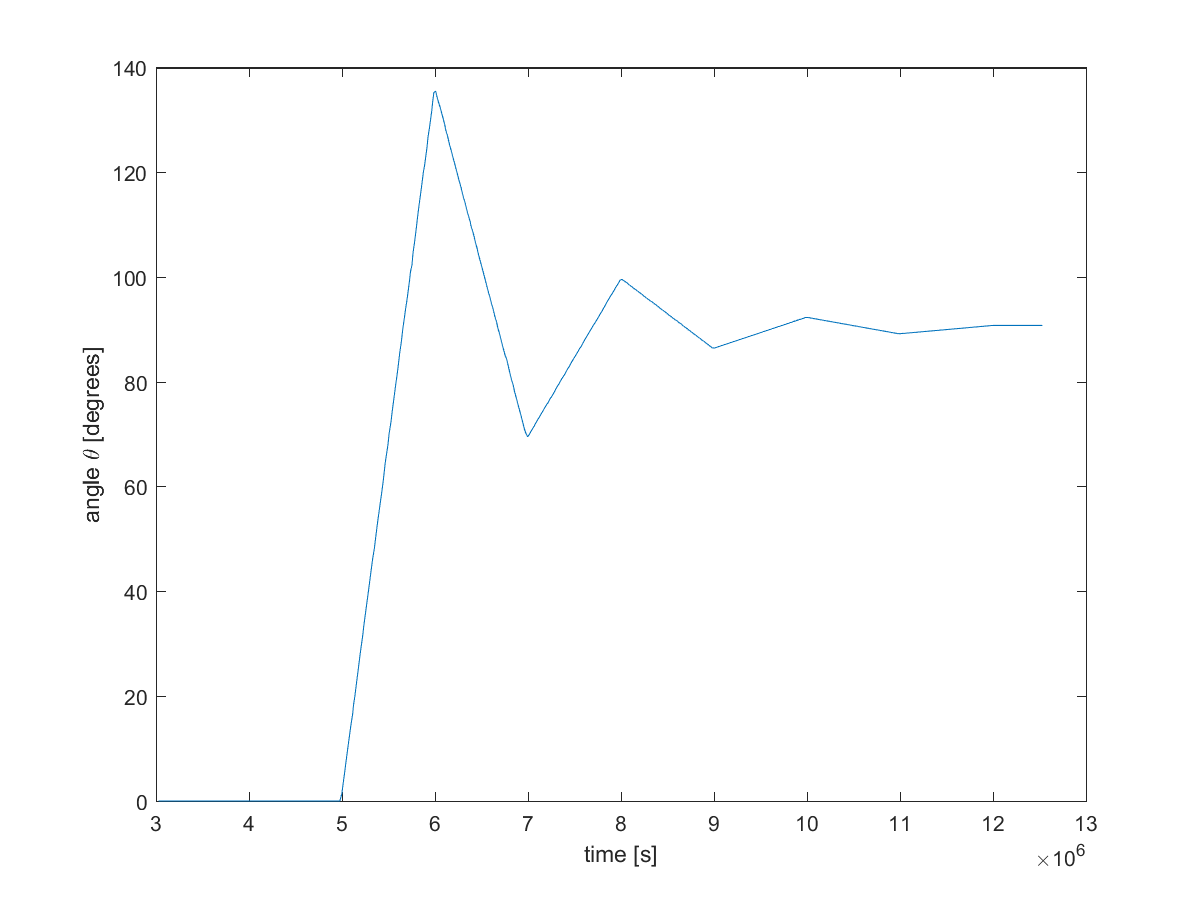
\includegraphics[scale = 0.5]{../matlab/images/task8_angleplot.png}
        \caption{Simulated rotation resonse.}
        \label{fig:task8_angleplot}
    \end{figure}
    \begin{figure}[H]
        \centering
        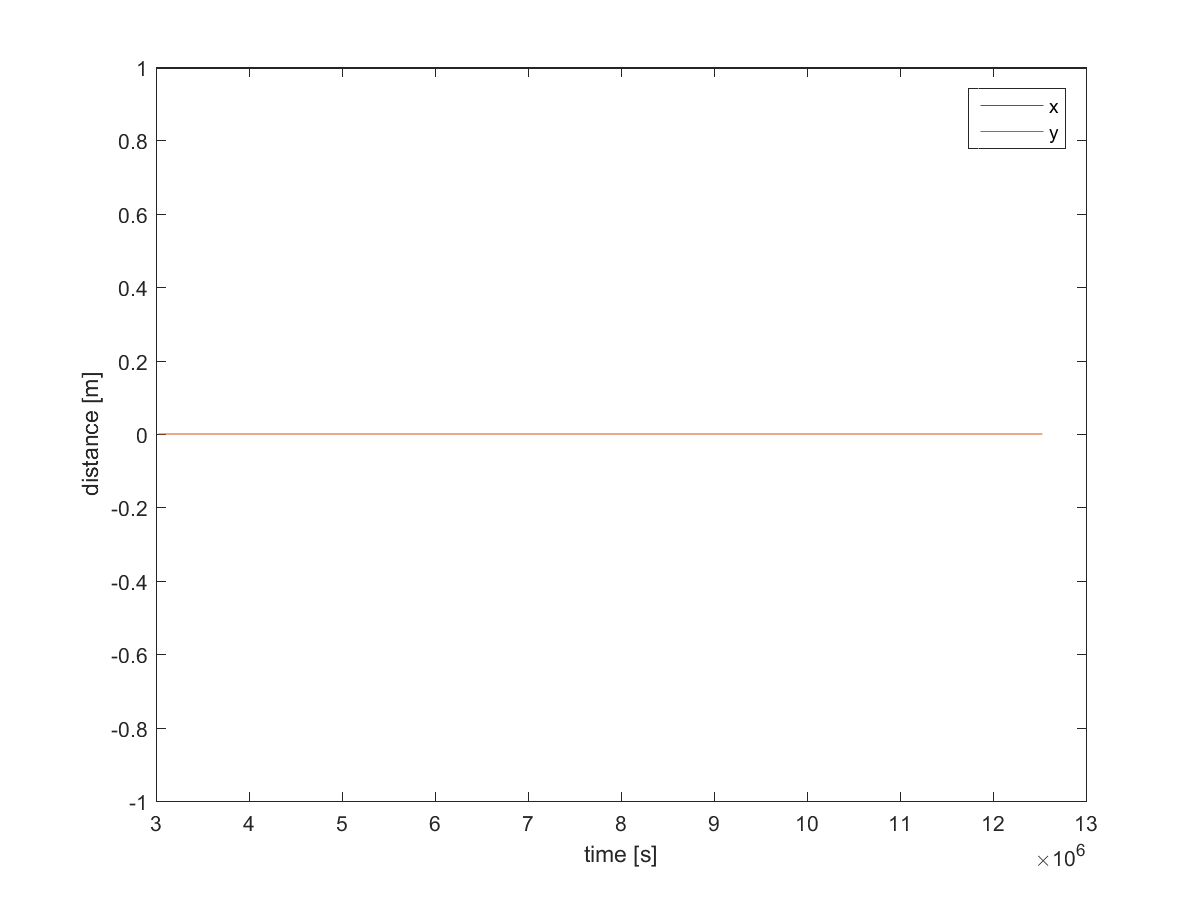
\includegraphics[scale = 0.5]{../matlab/images/task8_posplot.png}
        \caption{Simulated position response.}
        \label{fig:task8_posplot}
    \end{figure}
As can be seen, it is possible to maintain the angle at the desired value, as suggested by the fact that the poles of the system can be placed within the unit circle. When there is no translational movement, there are no disturbances in the angular controller, which allows for this exact control.
\section*{Task 9}
The equation 
	\begin{equation}
		\label{eq:omegasystem}
		d_0[k] = K_\omega(cos(\theta[k])(x_0-x[k]) + sin(\theta[k])(y_0-y[k]))
	\end{equation}
 	describes how $d_0$ depends on the angle desired angle and the current position. Using the given condition that $\theta[k] = \text{const.} := \theta$ and the controller in the task,
\begin{equation}
\label{eq:omegacontroller}
 	u_\omega [k] = K_\omega d_0 [k]
\end{equation} 	 
one can find the time dynamics of the system. Firstly, a unit time shift is employed, yielding
\begin{equation}
		d_0[k+\tau_s] = K_\omega(cos(\theta)(x_0-x[k]-x[k+\tau_s]) + sin(\theta)(y_0-y[k] - y[k+\tau_s)).
\end{equation}
Using equation (\ref{eq:xsystem}) and (\ref{eq:ysystem}) along with (\ref{eq:omegacontroller}), an expression for $d_0[k+1]$ can be reached,
\begin{equation}
d_0[k+1] = \left( 1 - K_\omega^2 \tau_s R (cos(\theta) + sin(\theta)) \right) d_0[k].
\end{equation}
For asymptotic stability, the pole should reside within the unit circle, leading to the criterion
\begin{equation}
\left|1 - K_\omega^2 \tau_s R (cos(\theta) + sin(\theta)) \right| <1,
\end{equation}
in turn giving the values for which the system is stable,
\begin{equation}
0 < K_\omega < \sqrt{\frac{2}{\tau_s R (cos(\theta) + sin(\theta))}}.
\end{equation}
The implementation in the controller is then done with a value of $K_\omega$ that is more conservative than the theoretical boundary, around 0.5-0.7 of the calculated value.
\section*{Task 10}
In Figure~\ref{fig:task10_stepplot} the performance of the controller is shown.
Figure~\ref{fig:task10_stepplot} shows that the controller is able to maintain its starting position. 
its starting position.  \begin{figure}[H]
        \centering
        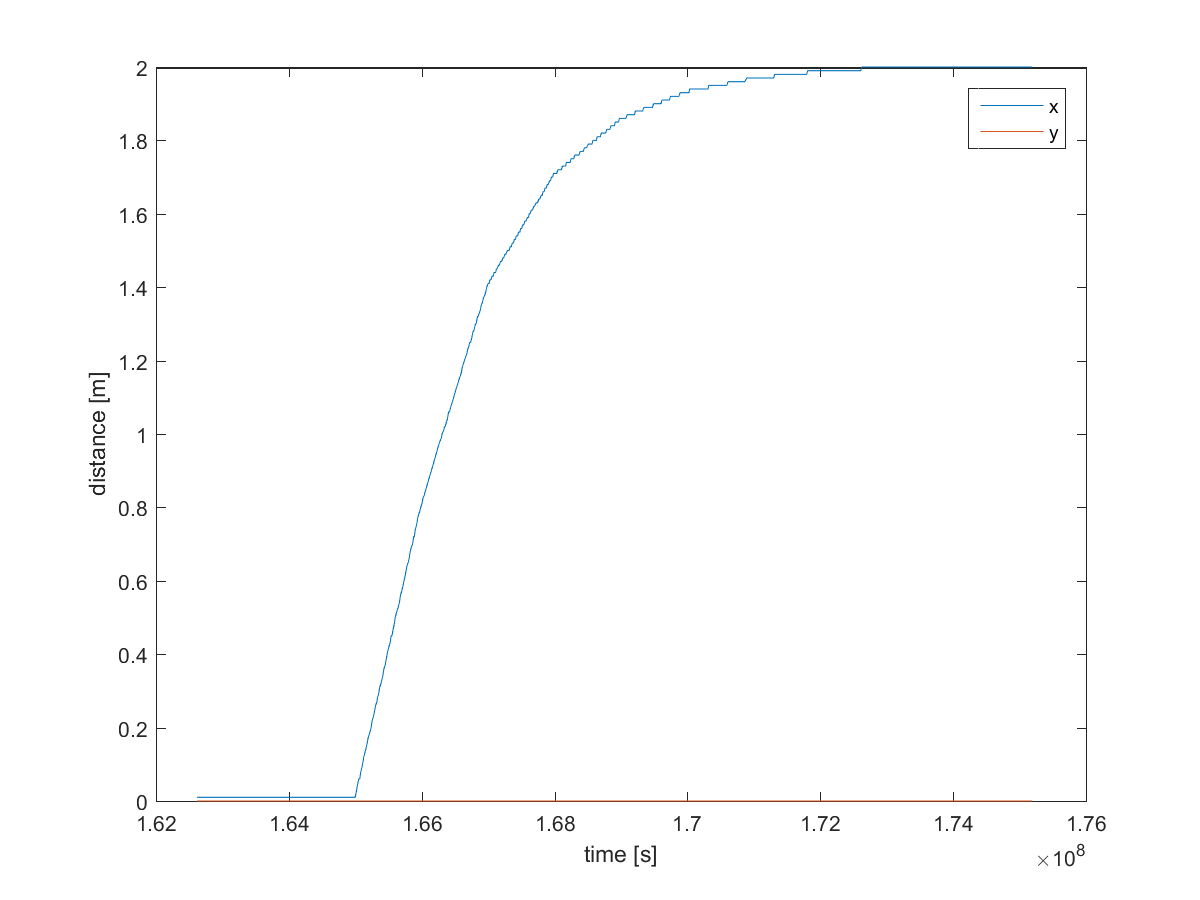
\includegraphics[scale = 0.5]{../matlab/images/task10_stepplot.png}
        \caption{Simulated position response when setting start to a different position.}
        \label{fig:task10_stepplot}
    \end{figure}
    
    \begin{figure}[H]
        \centering
        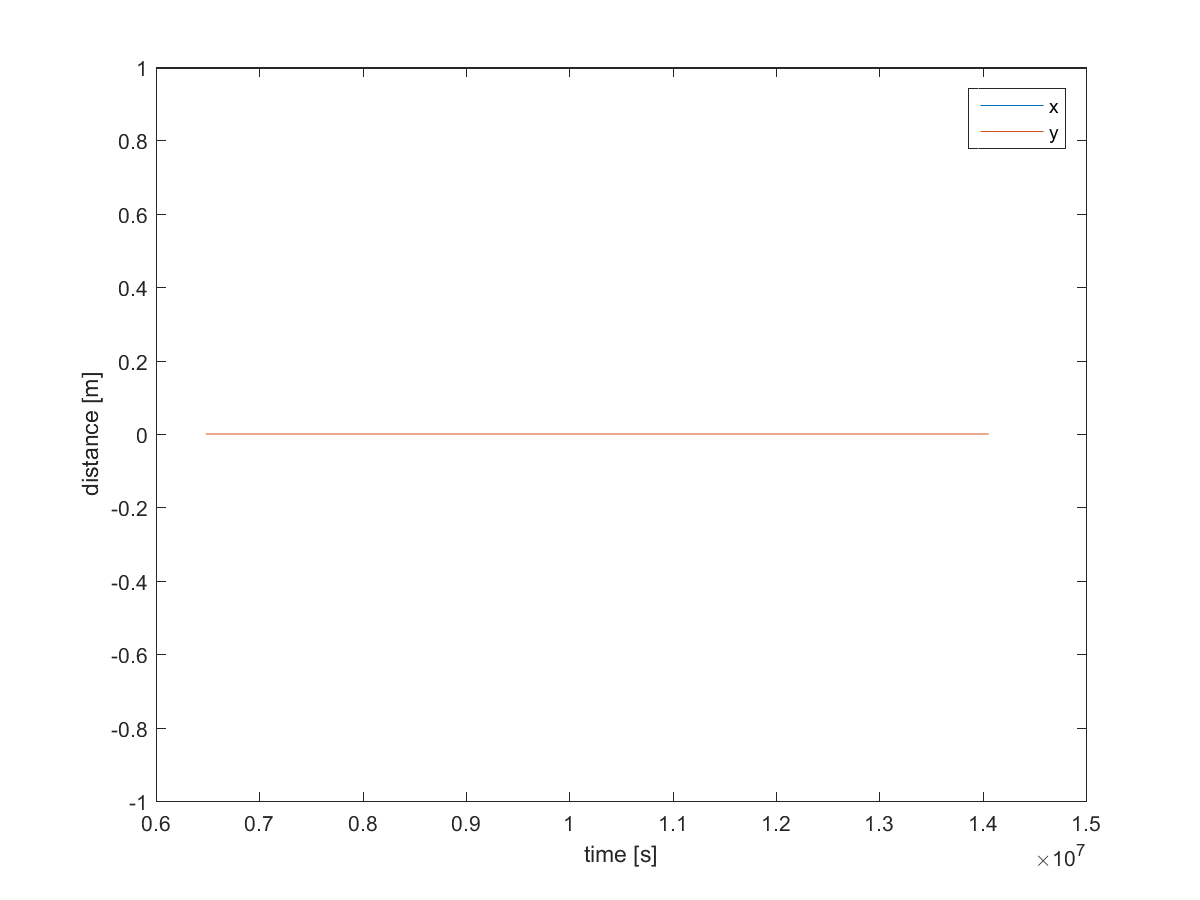
\includegraphics[scale = 0.5]{../matlab/images/task10_stillplot.png}
        \caption{Simulated position response when attempting to stand still.}
        \label{fig:task10_stillplot}
    \end{figure}
This could be possible because in theory the controller does not move in translational modes while turning.
\section*{Task 11}
In Figure~\ref{fig:task11_angleplot} the error $\theta^R - \theta[k]$ can be seen. In Figure~\ref{fig:task11_d0plot} $d_0$ can be seen.
\begin{figure}[H]
        \centering
        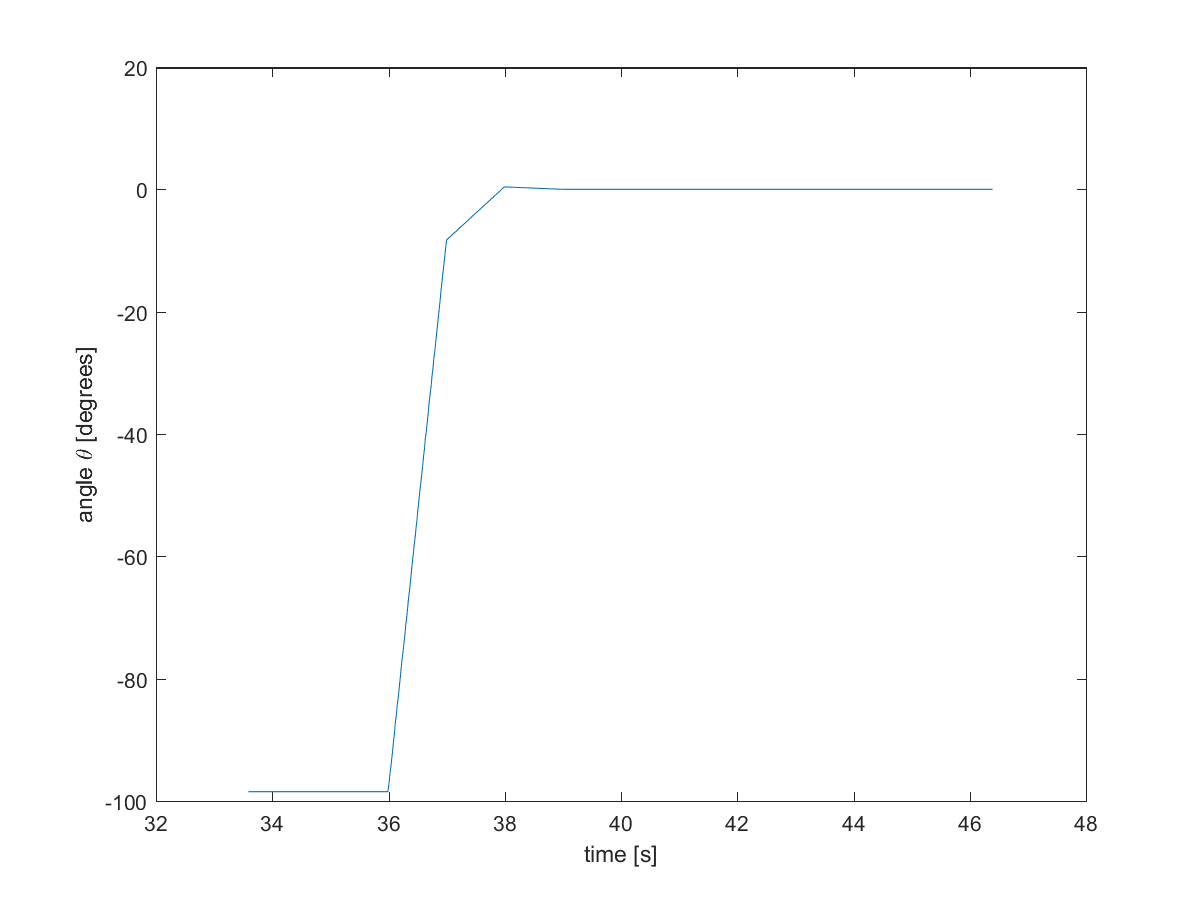
\includegraphics[scale = 0.5]{../matlab/images/task11_angleplot.png}
        \caption{Simulated angular response.}
        \label{fig:task11_angleplot}
    \end{figure}
    
    \begin{figure}[H]
        \centering
        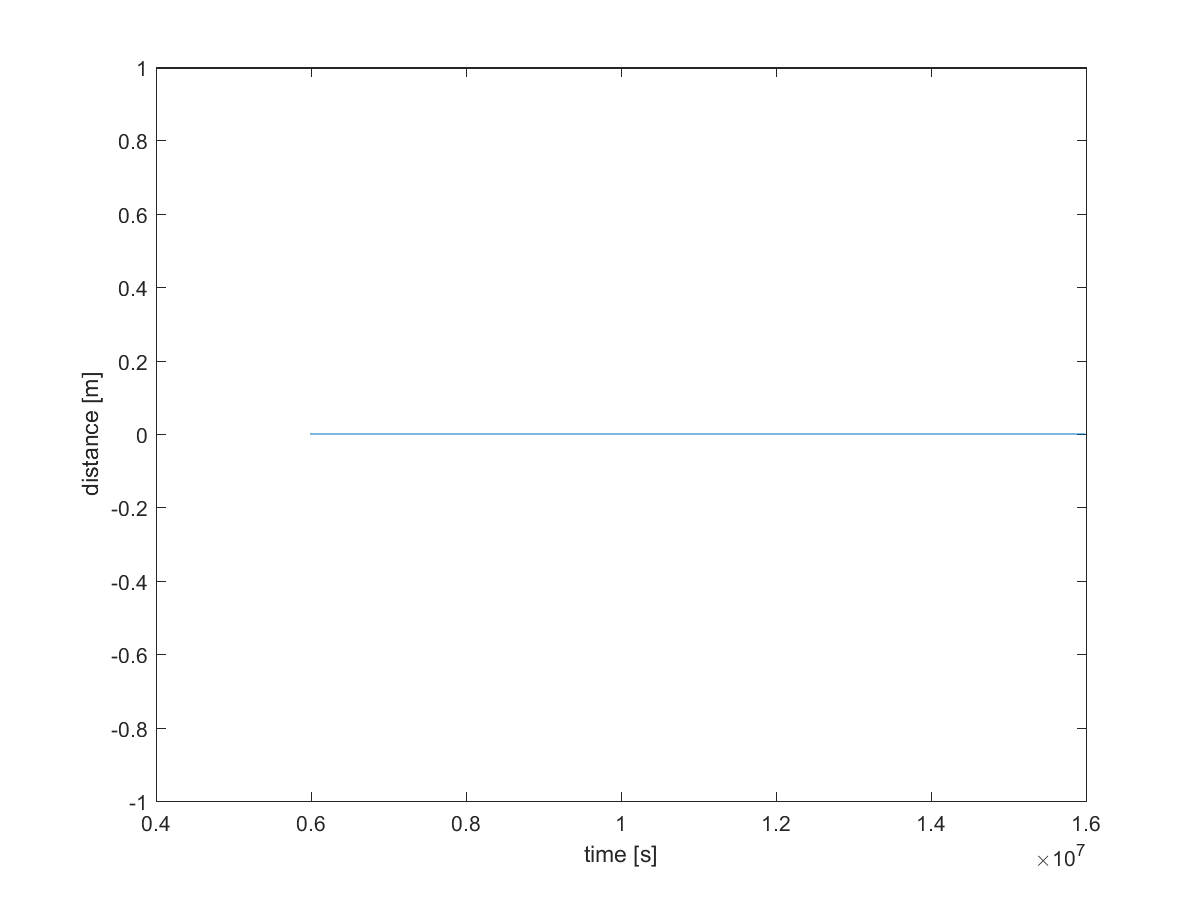
\includegraphics[scale = 0.5]{../matlab/images/task11_d0plot.png}
        \caption{Simulated position response.}
        \label{fig:task11_d0plot}
    \end{figure}
They evolve the same as when both controllers are engaged. This is most likely because in the simulation, the rotation is ideal and the position never leaves the origin. 
\section*{Task 12}
Given
\begin{equation}
d_g[k] = cos(\theta_g) (x_g - x[k]) + sin(\theta_g) (y_g - y[k])
\end{equation}
for the line follower, $d_g[k]$ is time shifted one step. The Euler forward equations (\ref{eq:xsystem}) and (\ref{eq:ysystem}) are substituted into the expression along with the controller
\begin{equation}
u_\omega[k] = K_\omega d_g[k]
\end{equation} 
yielding
\begin{equation}
d_g[k+1] = cos(\theta_g)(x_g - x[k] - \tau_s R K_\omega d_g[k] cos(\theta_g)) + sin(\theta_g)(y_g - y[k] - \tau_s R K_\omega d_g[k] sin(\theta_g)).
\end{equation}
Rewriting and using the  Pythagorean identity gives the final expression,
\begin{equation}
d_p[k+\tau_s] = (1 - \tau_s R K_\omega) d_p[k].
\end{equation}
With the criterion that the pole should be inside the unit circle, or
\begin{equation}
\left| 1 - \tau_s R K_\omega \right| < 1,
\end{equation}
gives the stability boundary for $K_\omega$,
\begin{equation}
0 < K_\omega < \frac{2}{\tau_s R}.
\end{equation}
\section*{Task 13}

 In figure \ref{fig:task13_positionplot} the position response can be seen.

\begin{figure}[H]
        \centering
        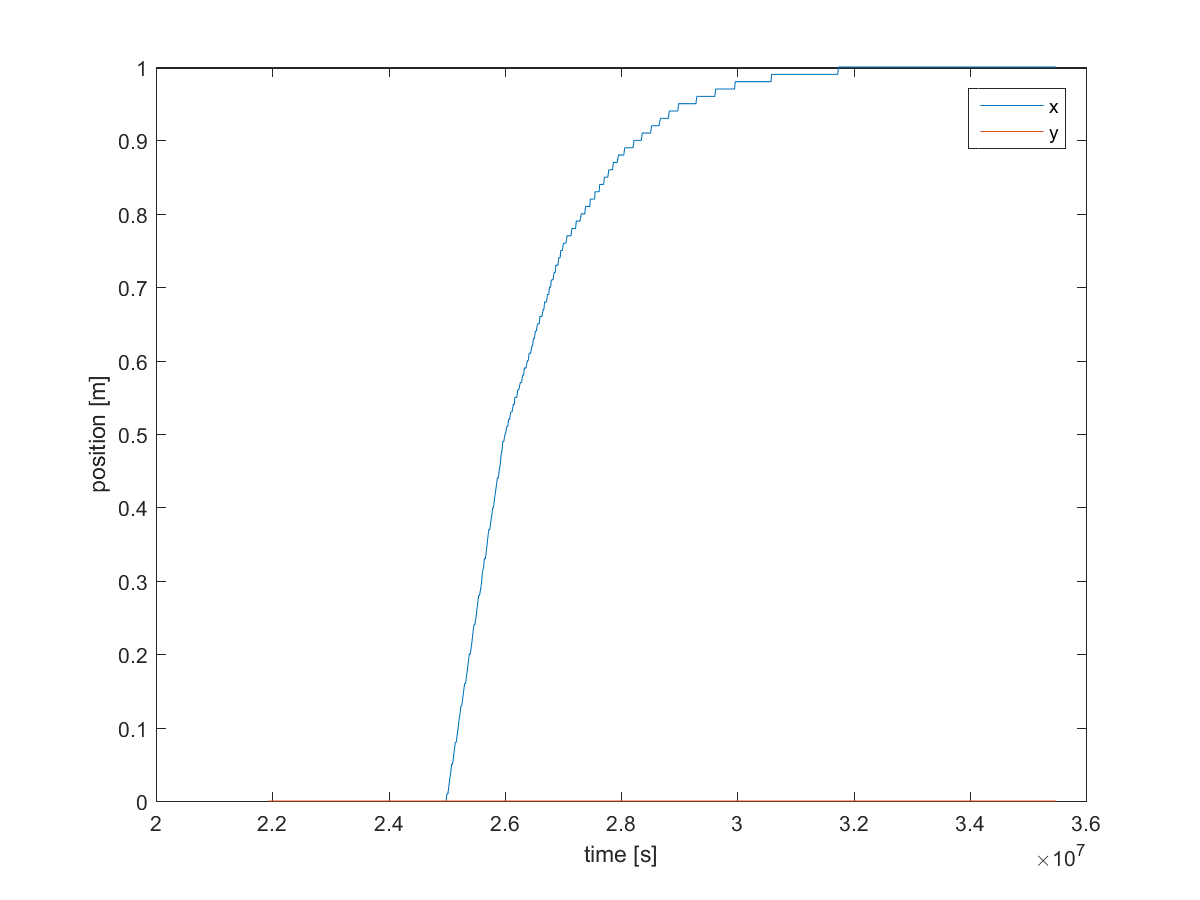
\includegraphics[scale = 0.5]{../matlab/images/task13_positionplot.png}
        \caption{Simulated position response.}
        \label{fig:task13_positionplot}
    \end{figure}
It is possible to reach the goal value, hinted by the fact that the system can be made asymptotically stable.
\section*{Task 14}

With the approximation given,
\begin{equation}
\label{eq:simplification}
d_p[k] = p(\theta[k] - \theta^g),
\end{equation}
one can time apply a time shift of one sampling time $\tau_s$ which will yield
\begin{equation}
\label{eq:timeshift}
d_p[k + \tau_s] = p(\theta[k + \tau_s] - \theta^g).
\end{equation}
Using the controller 
\begin{equation}
u_\psi[k] = K_\psi d_p[k]
\end{equation}
and pluggin into (\ref{thetadynamics}) and (\ref{eq:timeshift}) one gets
\begin{equation}
d_p[k + \tau_s] = \frac{p R K_\psi \tau_s}{L} d_p[k] + p(\theta[k] - \theta^g).
\end{equation}
Using (\ref{eq:simplification}) one yields the expression for the dynamics of the controller,
\begin{equation}
\label{eq:dp}
d_p[k+\tau_s] = \left ( 1 + \frac{p R K_\psi \tau_s}{L} \right ) d_p[k].
\end{equation}
The stability criterion for (\ref{eq:dp}) is given by the equation
\begin{equation}
\left | 1 + \frac{p R K_\psi \tau_s}{L} \right | < 1
\end{equation}
the place the pole inside the unit circle.
Allowing negative values, the values of $K_\psi$ for which the controller is stable are then bound by
\begin{equation}
-\frac{2L}{p R \tau_s} < K_\psi < 0.
\end{equation}
\section*{Task 15}
Looking at the simplification (\ref{eq:simplification}), the value of $p$ works like a proportional value in a P-controller. Thus, a higher $p$ makes the system faster but too large a value of $p$ may render the system unstable or cause overshoot.

\section*{Task 16}

  It is theoretically possible to have a controller that adjusts the robot
correctly if we are in continous time. Since we now are dealing with
descrete time it gets harder to adjust the robot perfectly. We would now
need some type of adjusting, non-uniform quantizer and sampler to get
the precision needed for our type of distances. This would have to
increse quantizing and sampling period the closer to $d_p[k]=0$ we would
get.
\begin{figure}[H]
    \centering
  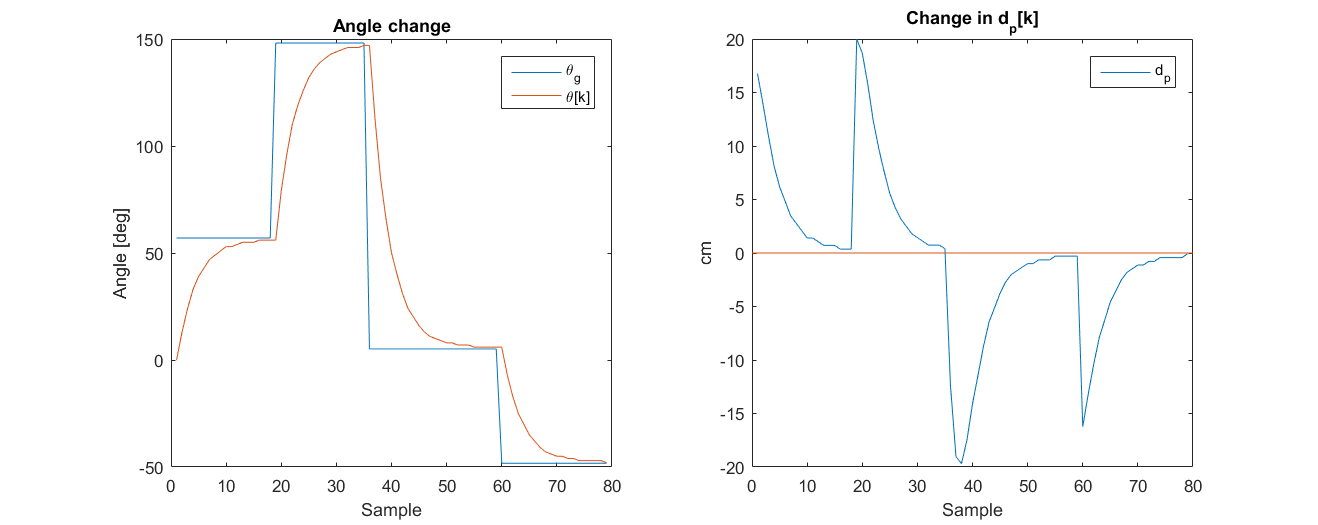
\includegraphics[width=\textwidth]{../matlab/images/task16.png}
  \caption{Control performance when $u_{\omega}=0$}
  \label{fig:task16}
\end{figure}

With the uniform quantizer and samplingtime that we have in our
simulations we get the results presented in figure \ref{fig:task16}. This shows
the control performance for the controller when $u_{\omega}=0$. Since
we cant get the preciseness needed to position the robot we can see that
it will not reach $\theta_g$ exactly but will stop rotating when the
threshold is reached. This is to prevent oscillation around $\theta_g$
which will occur if there is nothing to prevent adjustments when a good
enough presition is reached.

  
\section*{Task 17}

    They differ since they now need to recalculate the angle error when the
angle error gets to large. In Figure~\ref{fig:task17} we can see that
$d_p$ increses when the robot starts translation, it will then need to
correct itself on the move.

\begin{figure}[H]
    \centering
    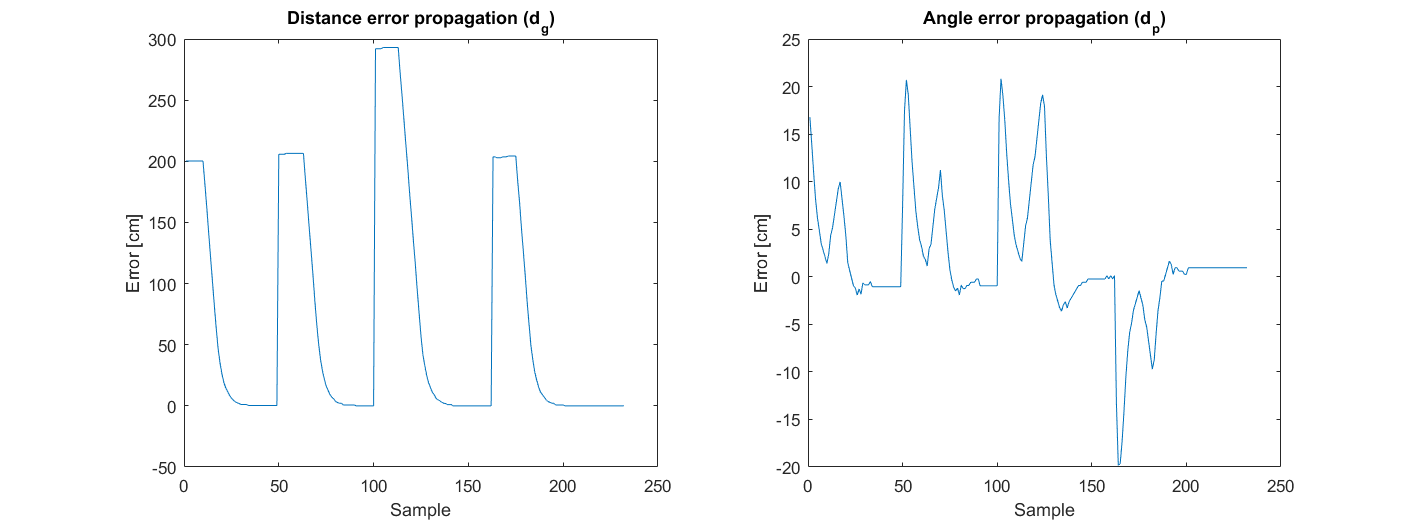
\includegraphics[width=\textwidth]{../matlab/images/task17.png}
    \caption{Control performance when both controllers is activated}
    \label{fig:task17}
\end{figure}


\section*{Task 18}

The hybrid automation is defined as,

\begin{equation}
    H = (Q,S,Init,f,D,E,G,R).
\end{equation}
We can model the controller with $Q$, the discrete state space $S$,
the continuous state space and initial states as,
\begin{align*}
    &Q=(Rotation,Translation,Goal)=(q_1,q_2,q_3) \\
    &S=\mathbb{R}^3 (x,y,\theta)\\
    &Init = Q \times \{ S \in \mathbb{R}^3 :x_0\wedge y_0 \wedge
    \theta_0\}
\end{align*} 
the vector fields, $f$ as,
\begin{align*}
    &f(q_1,S)=(Ru_{\omega}cos\theta,Ru_{\omega}sing\theta,R/Lu_{\Psi}) \\
    &f(q_2,S)=(Ru_{\omega}cos\theta,Ru_{\omega}sing\theta,R/Lu_{\Psi})\\
    &f(q_3,S)=(0,0,0),
\end{align*}
the domains, $D$ as,
\begin{align*}
    &D(q_1)=\{S\in \mathbb{R}^3:\theta \le r_1; |(x,y)-(x_0,y_0)|\le r_2\} \\
    &D(q_2)=\{S\in \mathbb{R}^3:|(x,y)-(x_g,y_g)| \le r_2\} \\
    &D(q_3)=\{S\in \mathbb{R}^3:|(x,y)-(x_g,y_g)| \le r_2\}
\end{align*}
the edges, $E$ as,
\begin{align*}
    &E = \{(q_1,q_2), (q_2,q_3), (q_3, q_1)\},
\end{align*}
the guards, $G$ as,

\begin{align*}
    &G_1(q_1,q_2)=\{\theta\in\mathbb{R}:\theta\le r_1\} \\
    &G_2(q_2,q_1)=\{\theta\in\mathbb{R}:\theta\le r_2\} \\
    &G_3(q_3,q_1)=\{Reset\}
\end{align*}
and the resets, $R$ as,
\begin{align*}
  &R(q_1,q_2,S)=R(q_2,q_3,S)=R(q_3,q_1,S)=\{S\}.
\end{align*}


\section*{Task 19}
  The state transitions can be seen in figure \ref{fig:task19_trans}
  where state 0 is rotating, state 1 is translation and state 2 is
  standstill. 

\begin{center}
    \begin{figure}[H]
      \centering
      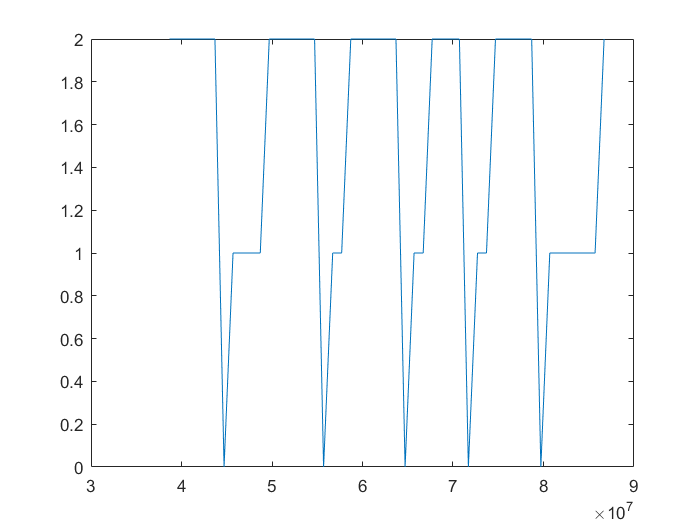
\includegraphics[scale = 0.5]{../matlab/images/task19_trans.png}
      \caption{State transitions for the controller between state 1, 2
      and 3}
      \label{fig:task19_trans}
    \end{figure}
\end{center}

This is when driving 1 $\rightarrow$ 3 $\rightarrow$ 6 $\rightarrow$ 5
$\rightarrow$ 8 $\rightarrow$ 1. This can also be seen in the plot in
figure \ref{fig:task13_positionplot} where the performance of the robot
can be seen.

\begin{center}
    \begin{figure}[H]
      \centering
      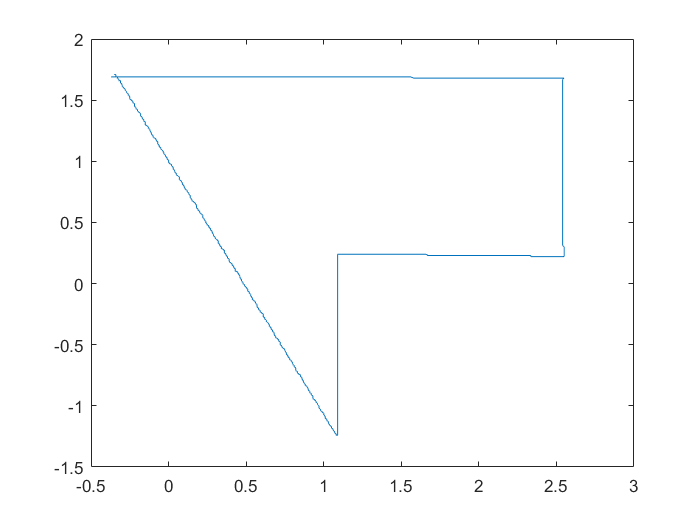
\includegraphics[scale=0.5]{../matlab/images/task19_cont.png}
      \caption{Control performance for the robot}
      \label{fig:task19_cont}
    \end{figure}
\end{center}

\section*{Task 21}

The difficulty comes from the delay between the computer and the
robot. There is a certain delay between when the user presses the button
and the robot responds.

\section*{Task 22}
The controller worked as it should in the simulations but did not work
when implemented in the physical system. More precisely, the rotational
controller worked when implemented but when the system switched state to
the line following part, it did not work. The simulation results when
following the track have been presented in Figure~\ref{fig:task19_cont}
and for the sake of completeness, the experimental results are
displayed in Figure~\ref{fig:task22}, though they do not contribute to the controller evaluation.
The group hypothesize that the controller might be flawed but working
during ideal conditions but when subjected to real life disturbances,
the low robustness of the control renders the system unstable and
unusable.

\begin{figure}[H]
    \centering
    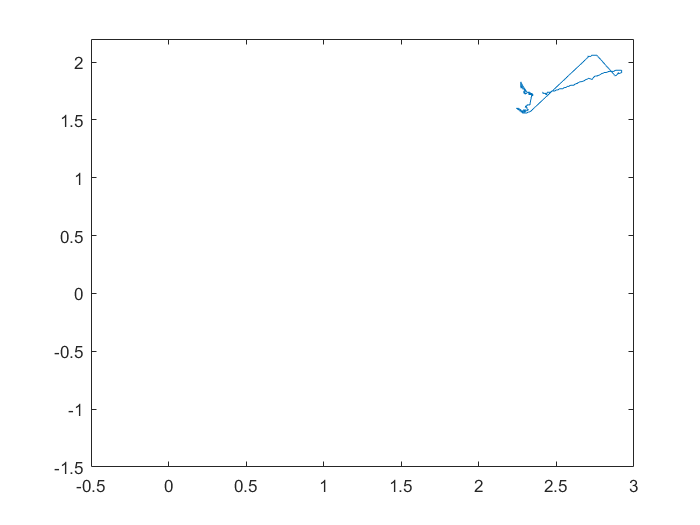
\includegraphics[scale=0.6]{../matlab/images/task22.png}
    \caption{The results for the robot during the lab}
    \label{fig:task22}
\end{figure}

\end{document}      % End of the document
